% !TeX root = ../beamer.tex
\section{Bistatisches Prinzip}

\begin{frame}
    \frametitle{Monostatische Geometrie}

    \begin{figure}
        \centering
        \begin{adjustbox}{max width=\textwidth,totalheight=\textheight-5\baselineskip}
            \begin{tikzpicture}
                
\coordinate (horizon) at (3,0);

\begin{scope}
    \clip (0,0) rectangle ({sqrt(2*pow(3,2))},{sqrt(2*pow(3,2))});
    \draw (0,0) circle [radius={sqrt(2*pow(3,2))}];
\end{scope}

\node [label={below:Radar}] (radar) at (0,0) {\Huge\faSatelliteDish};

\node [label={above:Target}] (target) at (3,3) {\Huge\faPlane};

\draw [<->,red] (radar) -- (target);
\draw [dotted] (radar) -- (horizon);

\pic [draw,angle radius=1.5cm,angle eccentricity=0.8,"$\phi$"] {angle=horizon--radar--target};

            \end{tikzpicture}
        \end{adjustbox}
        \caption{Monostatische Geometrie bei konventionellem Radar.}
    \end{figure}
\end{frame}

\begin{frame}
    \frametitle{Bistatische Geometrie}

    \begin{figure}
        \centering
        \begin{adjustbox}{max width=\textwidth,totalheight=\textheight-6\baselineskip}
            \begin{tikzpicture}
                % !TeX root = ../main.tex
\coordinate (rx1_coord) at (-2,0);
\coordinate (tx1_coord) at (2,0);
\coordinate (target_coord) at (1,1.25);

\node at (tx1_coord) [draw,fill=white] (tx1) {Tx};

\node at (rx1_coord) [draw,fill=white] (rx) {Rx};

\begin{scope}
    \clip
    let
    \p1=(target_coord),
    in
    (\x1 - 0.75cm,\y1 + 0.75cm) rectangle +(1.5,-1.5);
    \draw [color=gray]
    (2.42539052968,0) arc [start angle=0,end angle=360,x radius=2.42539052968,y radius=1.37204927807];
\end{scope}

\node at (target_coord) [label={[fill=white]above:Target}] (target) {\faPlane};

\draw [->,color=red] (tx1) -- node [black,midway,right,align=center] {$R_1$} (target);
\draw [->,color=red] (target) -- node [black,midway,left=4pt,align=center] {$R_2$} (rx);
\draw [->,color=blue] (tx1) -- node [black,midway,below,align=center] {$R_{\text{b}}$} (rx);

\pic [draw,angle radius=1cm,"$\beta$"] {angle=rx1_coord--target_coord--tx1_coord};

                \drawBistaticGeometry{bg}
            \end{tikzpicture}
        \end{adjustbox}
        \caption{Baseline \(R_{\text{b}}\), Entfernung: Sender/Ziel \(R_{1}\), Entfernung: Ziel/Empfänger \(R_{2}\), Bistatischer Winkel \(\beta\), Bewegungsrichtung Ziel \(\delta\), Geschwindigkeitsvektor \(v\).}
    \end{figure}
\end{frame}

\begin{frame}
    \frametitle{Bistatische Ellipse}

    \begin{figure}
        \centering
        \begin{adjustbox}{max width=\textwidth,totalheight=\textheight-5\baselineskip}
            \begin{tikzpicture}
                
\def\F{5}
\coordinate (rx1_coord) at (-\F,0);
\coordinate (tx1_coord) at (\F,0);
\coordinate (target_coord) at (2,3.5);
\coordinate (pencil) at (0.1,0.6);

\draw [visible on=<3->] (0,0)
let
\p1=($(target_coord)-(tx1_coord)$),
\p2=($(target_coord)-(rx1_coord)$),
\p3=(tx1_coord),
\n1={scalar((veclen(\x1,\y1) + veclen(\x2,\y2))*1pt/1cm)},
\n2={sqrt(pow(\n1/2, 2))},
\n3={sqrt(pow(\n1/2, 2) - pow(\F, 2))}
in
circle [x radius=\n2,y radius=\n3,draw=gray];

\draw [dotted] (rx1_coord) node [cross out,draw,solid] {} -- (0,0) node {\contour{bg}{$R_{\text{b}}$}} -- (tx1_coord) node [cross out,draw,solid] {};

\draw [visible on=<2->,dash dot] (rx1_coord) -- (target_coord) node [midway] {\contour{bg}{$R_{2}$}} -- (tx1_coord) node [midway] {\contour{bg}{$R_{1}$}};

\draw [visible on=<2->,<-] (target_coord) -- ++(pencil);

\node [visible on=<4->] at (0,-1.5) {%
    \(\begin{aligned}
            & R_{1} + R_{2}                & = \text{const.} & \dots \text{bistatische Summe}      \\
        R = & R_{1} + R_{2} - R_{\text{b}} & = \text{const.} & \dots \text{bistatische Entfernung} \\
    \end{aligned}
    \)};

            \end{tikzpicture}
        \end{adjustbox}
        \caption{Zeichenregeln einer bistatischen Ellipse.}
    \end{figure}
\end{frame}

\begin{frame}
    \frametitle{Bistatische Ellipsoid}

    \begin{figure}
        \centering
        \begin{adjustbox}{max width=\textwidth,totalheight=\textheight-6\baselineskip}
            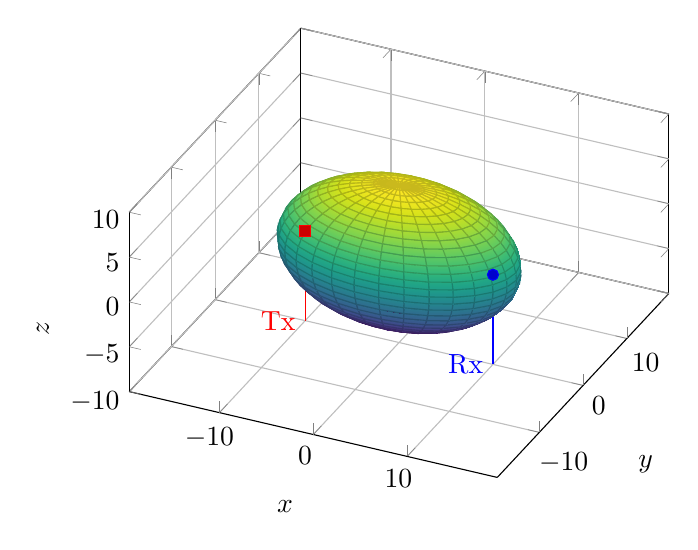
\begin{tikzpicture}
                % !TeX root = ../main.tex
\def\R{25}
\def\F{10}
\def\a{sqrt((\R/2)^2)}
\def\b{sqrt((\R/2)^2 - \F^2)}
\def\c{\b}
\def\xmin{-int(\a + 5 - mod(\a - 5, 5))}
\def\ymin{-int(\b + 5 - mod(\b - 5, 5))}
\def\zmin{-int(\c + 5 - mod(\c - 5, 5))}
\def\xmax{+int(\a + 5 - mod(\a - 5, 5))}
\def\ymax{+int(\b + 5 - mod(\b - 5, 5))}
\def\zmax{+int(\c + 5 - mod(\c - 5, 5)))}
\begin{axis}[
        z buffer=sort,
        axis equal,
        colormap/viridis,
        samples=31,
        xmin=\xmin,
        ymin=\ymin,
        zmin=\zmin,
        xmax=\xmax,
        ymax=\ymax,
        zmax=\zmax,
        xlabel=$x$ \si{\kilo\metre},
        ylabel=$y$ \si{\kilo\metre},
        zlabel=$z$ \si{\kilo\metre},
        grid=major,
        view/az=25,
        view/el=30,
    ]
    \addplot3 coordinates {
            (\F,0,0)
            (\F,0,\zmin)
        } node[left,pos=0] {Rx};
    \addplot3 coordinates {
            (-\F,0,0)
            (-\F,0,\zmin)
        } node[left,pos=0] {Tx};
    \addplot3 [
        surf,
        shader=faceted interp,
        opacity=1,
        domain=0:180,
        y domain=0:360,
    ] (
    {\a*sin(x)*cos(y)},
    {\b*sin(x)*sin(y)},
    {\c*cos(x)}
    );
\end{axis}

            \end{tikzpicture}
        \end{adjustbox}
        \caption{Exemplarischer bistatischer Ellipsoid für \(R = \SI{5}{\kilo\metre}\) and a baseline of \(R_{\text{b}} = \SI{20}{\kilo\metre}\). Daraus resultiert eine bistatische Summe von \(R_{\text{S}} = \SI{25}{\kilo\metre}\).}
    \end{figure}
\end{frame}

\begin{frame}
    \frametitle{Bistatische Geschwindigkeit}

    Notwendigkeit der Geschwindigkeitsbestimmung:
    \begin{itemize}
        \item \textbf{Clutter-Filtering} (Terrain, Bäume, Gebäude, Vögel, etc.)
        \item Erlaubt \textbf{Differenzierung} verschiedener Objekttypen
    \end{itemize}

    Allgemeine Definition der \textbf{bistatischen Geschwindigkeit}:
    \begin{itemize}
        \item Die augenblickliche Veränderung der bistatischen Entfernung in der Zeit.
              \begin{equation}
                  V = \frac{d}{d t} R
              \end{equation}
    \end{itemize}

\end{frame}

\note[itemize]{
    \item Bistatische Geschwindigkeit nicht linear proportional zu kartesischer Geschwindigkeit!!!
}

\begin{frame}
    \frametitle{Bistatische Geschwindigkeit}

    Wesentlich Nützlicher:
    \begin{itemize}
        \item Messung aus Dopplershift (\(\lambda\) \dots Wellenlänge, \(f_{d}\) \dots Dopplerfrequenz)
              \begin{equation}
                  V = - \lambda f_{d}
              \end{equation}
        \item Negatives Vorzeichen, da Geschwindigkeit \textbf{positiv} wenn Objekt sich \textbf{weg bewegt}.
    \end{itemize}

\end{frame}

\note[itemize]{
    \item \(f_{d} = f - f_{0}\)
    \item D.h.: Objekt bewegt sich weg -> Rotverschiebung -> tiefere Frequenz am Empfänger -> \(f_{d} < 0\)
    \item Andersherum: Objekt bewegt sich zu uns -> Blauverschiebung -> höhere Frequenz am Empfänger -> \(f_{d} > 0\)
}

\begin{frame}
    \frametitle{Relation: Bistatische Geschw.\ vs.\ Kartesische Geschw.}

    \begin{figure}
        \begin{adjustbox}{max width=\textwidth,totalheight=\textheight-5\baselineskip}
            \begin{tikzpicture}
                
\def\F{5}
\coordinate (l_foci_coord) at (-\F,0);
\coordinate (r_foci_coord) at (\F,0);
\coordinate (point_on_ellipse_coord) at (6,0);

\draw (0,0)
let
\p1=($(point_on_ellipse_coord)-(r_foci_coord)$),
\p2=($(point_on_ellipse_coord)-(l_foci_coord)$),
\n1={scalar((veclen(\x1,\y1) + veclen(\x2,\y2))*1pt/1cm)},
\n2={\n1/2},
\n3={sqrt(pow(\n1/2, 2) - pow(\F, 2))}
in
circle [x radius=\n2,y radius=\n3,draw=gray];

\draw [dotted] (l_foci_coord) node [cross out,draw,solid] {} -- (0,0) node {\contour{bg}{$R_{\text{b}}$}} -- (r_foci_coord) node [cross out,draw,solid] {};

\foreach \u in {-5.5,-5,...,5.5} {
        \draw [->,blue] let
        \p1=($(point_on_ellipse_coord)-(r_foci_coord)$),
        \p2=($(point_on_ellipse_coord)-(l_foci_coord)$),
        \n1={scalar((veclen(\x1,\y1) + veclen(\x2,\y2))*1pt/1cm)},
        \p3=(\u,{sqrt( (pow(2 * \F / \n1, 2) - 1) * pow(\u, 2) + pow(\n1 / 2, 2) - pow(\F, 2) )}),
        \p4=($(\p3)!1cm!(l_foci_coord)$),
        \p5=($(\p3)!1cm!(r_foci_coord)$),
        \p6=($(\p4) + (\p5) - (\p3)$),
        in
        (\p3) -- ($(\p6)!1.5!(\p3)$);
    }

\foreach \u in {-6,6} {
        \draw [->,blue] let
        \p1=(\u,0),
        \p2=($(\p1)!1cm!(l_foci_coord)$),
        \p3=($(\p1)!1cm!(r_foci_coord)$),
        \p4=($(\p2) + (\p3) - (\p1)$),
        in
        (\p1) -- ($(\p4)!1.5!(\p1)$);
    }

\foreach \u in {-5.5,-5,...,5.5} {
        \draw [->,blue] let
        \p1=($(point_on_ellipse_coord)-(r_foci_coord)$),
        \p2=($(point_on_ellipse_coord)-(l_foci_coord)$),
        \n1={scalar((veclen(\x1,\y1) + veclen(\x2,\y2))*1pt/1cm)},
        \p3=(\u,{-sqrt( (pow(2 * \F / \n1, 2) - 1) * pow(\u, 2) + pow(\n1 / 2, 2) - pow(\F, 2) )}),
        \p4=($(\p3)!1cm!(l_foci_coord)$),
        \p5=($(\p3)!1cm!(r_foci_coord)$),
        \p6=($(\p4) + (\p5) - (\p3)$),
        in
        (\p3) -- ($(\p6)!1.5!(\p3)$);
    }

            \end{tikzpicture}
        \end{adjustbox}
        \caption{Vektoren in Richtung maximaler bistatischer Geschwindigkeit.}
    \end{figure}

\end{frame}
